\chapter{Overview}\label{s:overview}
\todo{check if overview matches with Implementation and covers all BG and Concerns}

This overview contains a Utility Tree, which captures the Architecturally significant requirements (ASR). These ASRs are extracted from interviews (interviewee description in Appendix  \ref{Appendix A}) and combine with the Business Goals and Concerns (available in Appendix \ref{Appendix B} and  \ref{Appendix C}) 

\graphicspath{ {./images/} }
\begin{figure}
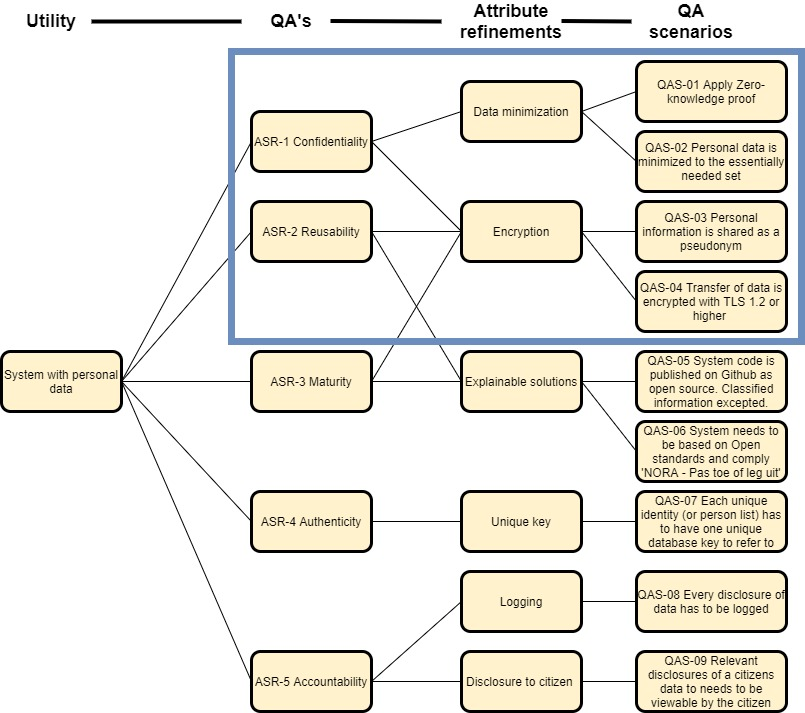
\includegraphics[width=14cm]{Decomposition of ASR and QAS-Utility Tree v3.jpg}\\
\caption{Decomposition of Architecturally significant requirements}
\label{fig:ASR1}
\end{figure}

\begin{table}[h!]
\centering
\begin{tabular}{||l l l||} 
 \hline
 Business Goal(s) (BG) & Concern(s) (C) & Architectural Significant Requirement (ASR) \\ [0.5ex] 
 \hline\hline
 \makecell {BG-03} & C-03 & ASR-1 Confidentiality \\
 \hline
 \makecell {BG-01, BG-02} & C-01, C-02 & ASR-2 Re-usability\\
\hline
 \makecell {BG-05} &  C-09 & ASR-3 Maturity  \\
 \hline
\makecell {BG-04} & C-04, C-05, C-06, C-11 & ASR-4 Authenticity \\
 \hline
 \makecell {BG-01} & C-10 & ASR-5 Accountability  \\ [1ex] 
 \hline
\end{tabular}
\caption{ASRs Plotted on business goals and concerns.}
\label{ASR_BG_C}
\end{table}

Concerns C-07, C-08 and C-11 and BG-06 are not addressed in this overview, because the scope of this research is not taking in account laws, exceptions and non-government organizations. However, these concerns are considered possible relevant for future research and therefore included in the appendix.


% \todo{
% This section provides a high-level outline of the proposed system or solution.
% It typically illustrates the system architecture or the interactions between the
% different solution components (via a “boxes-and-arrows” diagram) from a user’s
% perspective.
% }